\section{Overview}\label{overview}

\emph{This section is co-authored with Marissa Allen}

We set out to create a tool that would help people design 3D pop-up
cards. We were driven by our own struggles in creating 3D pop-up cards
and the desire to create an original design without a template. As we
progressed in our project, we began to focus on developing a tool that
would provide a way to create pop-ups more intuitively, without
explicitly understanding how to create a valid 90-degree pop-up card.
Our tool allows users to design, iterate, and preview an original pop-up
card before they even pick up a pair of scissors.

\subsection{Technical Overview}\label{technical-overview}

Our algorithmic simulation and validity detection is based on a tight
set of constraints to the pop-up card problem. We require the card to
have a central main valley fold --- from there we can determine the
orientation, as alternating folds fold in opposite orientations. The
card then folds 180 degrees; this implies parallelogram constraints
between all the edges in a sideways cross-section (with the exception of
v-fold features).

All fold endpoints must have cuts between them --- although these cuts
can be arbitrary shapes. Cuts can also form holes (regions bounded by
cuts). All folds and cuts are generated by a user-selected fold feature
(a pre-defined type of fold or shape that meets validation
requirements). The 3D meshes are constructed from individual planes
which are defined as any surface between cuts and folds. Based on the
folds, these are then oriented and translated based on the angle of the
main driving fold joint. We rotate 3D mesh planes to animate the folding
process. Each of the section planes is translated in relation to the
plane oriented above the fold and rotated in relation to the main
driving joint.

Our approach constructs a tree representation of the planes based on
fold adjacency and uses this for determining the parent child
relationships in the simulated 3D view. We also use a tree-based
structure to store associations between logical geometric units.

\subsection{Pipeline Overview}\label{pipeline-overview}

To begin, a user draws a design using the fold feature tools: box fold,
polygon, freeform and v-fold. These tools create a pattern of cuts and
folds, displaying an interactive preview of the design as the user
creates it. The cuts and folds created with these tools remain
associated with each other, and can be modified or deleted as a unit.

Each time a new shape is added to the design, it is evaluated for
validity: whether it can fold to 90 degrees and be parsed into
individual planes. The planes are then linked together in an acyclic
graph based on the planes' abutting top edges. This acyclic graph allows
us to shade planes based on orientation in 2D and simulate the design in
3D. Each feature can also be modified or deleted, by tapping on the
feature an selecting an entry from the list of available options.

This process continues until the user decides to preview the design in
3D. The 3D preview displays a preview of how the design will fold, which
can be manipulated using a pinch gesture. The user is free to return to
the 2D drawing interface and continue editing his/her design or save the
design as either a raster file or SVG vector file. After this step, the
user can print and cut the raster file or open the SVG file on a laser
cutter or other cutting tool. We automatically save designs locally when
leaving the design workspace, so users can restore their work.

\subsection{Development Process}\label{development-process}

We designed and developed the software interactively, frequently testing
prototypes with users. The full source for our software is available on
github.com, at \url{http://github.com/harquail/foldlings/}.

\begin{figure}[htbp]
\centering
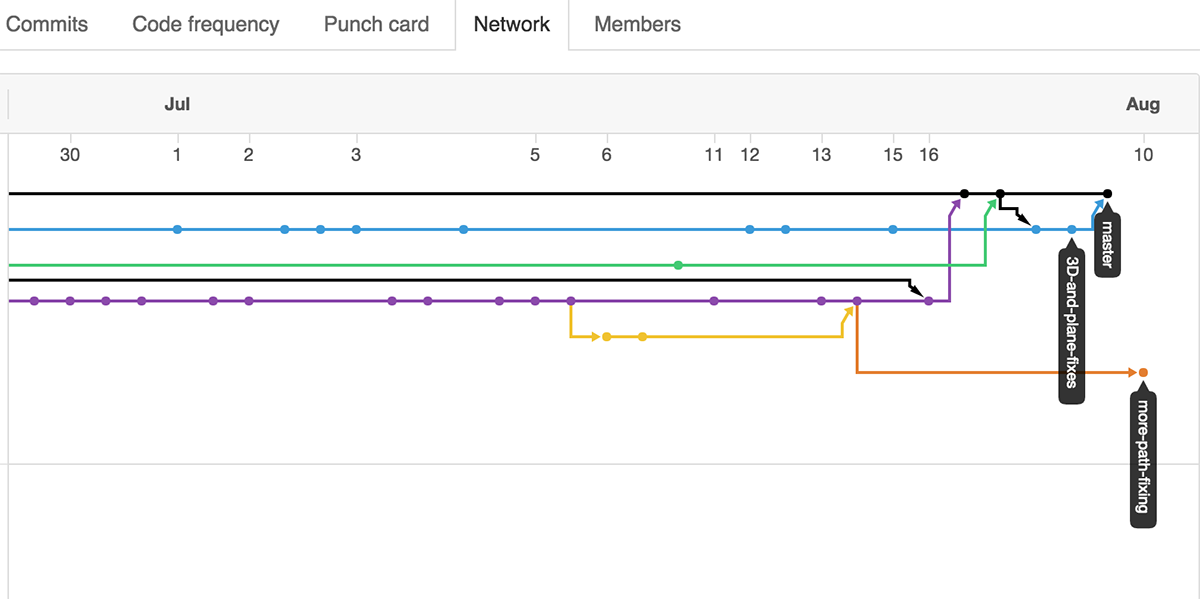
\includegraphics{figures/30_UI_Design_Philosophy/gitflow.png}
\caption{We used github to build Foldlings collaboratively. Our workflow
involved creating new code branches for each feature, and reviewing the
changes before merging back into the master branch of the codebase.}
\end{figure}
